% 제7회 한국 인공지능 학술대회 (KICS 인공지능소사이어티) 투고 원고
\documentclass[a4paper,twocolumn,9pt]{extarticle}
\usepackage{kotex}
\usepackage[margin=1.7cm,top=1.9cm,bottom=1.6cm]{geometry}
\usepackage{graphicx}
\usepackage{amsmath}
\usepackage{setspace}
\usepackage[font=small,skip=3pt]{caption}
\usepackage{xcolor}
\usepackage[hidelinks]{hyperref}   % 인용·그림 번호 클릭 시 해당 위치로 점프

\newcommand{\new}[1]{\textcolor{red}{#1}}
\newcommand{\term}[1]{\textcolor{blue}{#1}}  % 용어 통일 감사용 (임시)
\newcommand{\rev}[1]{\textcolor{violet}{#1}}  % 윤문·수치복원 표시 (임시)
\setlength{\columnsep}{0.6cm}
\pagestyle{empty}


\renewcommand{\thesection}{\Roman{section}.}
\makeatletter
\renewcommand\section{\@startsection{section}{1}{\z@}%
  {1.2ex plus .5ex}{0.8ex plus .3ex}{\normalsize\bfseries}}
\makeatother

\begin{document}


\twocolumn[{
\begin{center}
{\large\bfseries Title}\\[1.2ex]
{박경태, 김상우, 오윤선$^{\dagger}$}\\
{한양대학교}\\[0.6ex] 
{\small rudxo1997@hanyang.ac.kr, kimz1121@hanyang.ac.kr, $^{\dagger}$yoh21@hanyang.ac.kr}\\[2.0ex] 
{\large\bfseries Title}\\[1.2ex]
{Kyungtae Park, Sangwoo Kim, Yoonseon Oh$^{\dagger}$}\\ 
{Hanyang University.}\\[2.0ex]
{\bfseries 요 약}
\end{center}
\begin{quote}\small
Vision-Language-Action(VLA) 모델이 작업을 수행할 때 스스로 현재 어떤 \term{작업 단계(action phase)}를 진행중인지를 우리가 알 수 있다면, 이는 VLA모델에 대한 설명가능성과 추론 시 제어 및 개입의 출발점이 된다. 본 연구는 모델이 현재 수행 중인 \term{phase}를 내부 activation에서 판독할 수 있음을 보인다. GR00T N1.5의 action head(DiT)의 residual stream activation을 라벨 없이 clustering하면, 각 cluster는 특정 \term{primitive action phase}에 국한되어 나타나고 다른 \term{phase}에서는 잘 나타나지 않는다. 이 대응을 이용하면 학습에 사용하지 않은 scene에서도 activation 한 스텝만으로 현재 \term{phase}를 정확도 0.82로 읽을 수 있으며, 이는 진행 시간만 쓰는 시간 대조군과 외부 관찰 기반 행동 이벤트 대조군을 웃돈다. Cluster는 사람이 정의한 \term{phase}보다 더 잘게 나뉘지만, 각 조각이 \term{phase}에 대해 순수하기 때문에 판독이 성립한다. \rev{이 구조는 압축 모델을 AE에서 SAE로 바꾸어도, 독립적으로 재수집한 데이터에서도 재현된다.} 즉, VLA activation에는 \term{phase}와 정합적인 구조가 존재해 추론 중 online detection이 가능하며, 본 논문에서 이를 unseen scene에서 평가하여 확인하였다.
\end{quote}
\vspace{0.8ex}
}]

\begin{figure*}[!t]
  \centering
  
\includegraphics[width=0.70\textwidth]{figs/fig1_purity_residual.pdf}
  \caption{\rev{(a) cluster$\times$GT \term{phase} contingency(PPCC candle, k=8). 최빈 \term{phase}로 행을 정렬하면 블록-대각 구조가 나타난다(순도 0.888). (b) scene 잔차화 후에도 \term{phase} margin은 유지되고, (c) scene MI는 급감한다.}}
  \label{fig:purity}
\end{figure*}
\section{서 론}
VLA 모델은 내부 상태를 이해하기 힘든 블랙박스이지만 실제 로봇을 조작하므로, 모델이 지금 무슨 작업을 진행 중이라고 인지하는지 사람이 파악할 수 있어야 한다는 설명 가능성이 특히 중요하다. 본 논문에서 \term{action phase}란 manipulation task를 의미 단위로 나누었을 때 로봇이 수행하고 있는 하위 작업(subtask)을 의미한다. 예컨대 Pick \& Place task는 reach, grasp, transport, place의 \term{phase}로 구성된다\cite{options}. 이러한 현재 \term{phase}를 파악하는 방법에는 외부 관찰자가 카메라나 기타 센서들을 활용해 로봇의 현재 상태나 궤적 같은 외부 관찰 정보를 활용하는 방법이 있다\cite{lotus}. 하지만 외부 관찰은 로봇이 겉보기에 무엇을 하는지 알려줄 뿐이며, 모델이 스스로 어떤 작업을 하고 있다고 인지하는지, 즉 내부 표상이 가리키는 \term{phase}는 내부 activation을 직접 읽어야만 알 수 있고, 이는 겉보기 행동과 어긋났을 때 수정을 위한 전제 조건이다. VLA 내부 표현을 해석하려는 최근 시도들은
Sparse Auto Encoder(SAE)로 residual stream에서 grasp, transport와 같은 primitive action에 대응하는 feature를 찾아내거나\cite{saevla,egsae}, linear probe로 layer별 상태를 관측하고 그 방향으로 activation steering을 적용해 행동을 제어할 수 있음을 보였다\cite{observing,mechinterp}. \rev{그러나 이들은 발견된 feature가 언제 활성화되는지를 사람이 rollout 영상과 대조해 수동으로 이름을 붙이는 데 그치며, 내부 표상이 사람이 정의한 phase를 얼마나 정확히, 어떤 단위로 담고 있는지는 정량화하지 않는다.} VLA의 내부 \term{phase}를 추론 중에 online으로 읽을 수 있으면 설명을 넘어 조건부 개입이나 실패감지\cite{safe}의 조건신호로 활용할 수 있다. 본 연구는 GR00T N1.5\cite{groot}가 RoboCasa\cite{robocasa} 주방 조작을 수행하는 동안의 activation을 Autoencoder(AE)와 clustering으로 분석해, 모델 내부 \term{phase}가 사람이 정의한 \term{phase}와 갖는 관계를 Mutual Information(MI)로 정량화한다. 

\section{방 법}
\textbf{Data. } RoboCasa 주방 조작 환경에서 GR00T N1.5의 rollout을 수집한다. 대상은 5개 task(OpenDrawer, PnPCounterToCab, OvenRack, DishwasherRack, CoffeeSetupMug)에 속하는 10개 instruction이며, instruction마다 10개 scene에서 10회씩 총 100회의 rollout을 수집하였다. \rev{모델이 1회 추론 할 떄 마다 action expert의 resudual sttream activation을 캡쳐한다. 모델은 추론당 16개의 action step을 추론하며 그중 5개 action을 환경에서 실행하도록 세팅하였다. 이 activation은 12번째 layer의 마지막 denoising step에서 49개 토큰을 평균한 스텝당 1{,}536차원 벡터이고, GT \term{phase} 라벨도 같은 시점에서 읽는다.}

\rev{Detector의} 학습과 평가는 scene 단위로 분리한다. 10개 scene 중 8개를 학습용, 2개를 평가용으로 나누고, 이러한 분할을 무작위로 3가지 구성한다. 분할마다 표준화, AE, clustering, \term{phase} 매핑을 학습 scene만으로 새로 적합하며, 세 분할의 평가 결과를 평균해 보고한다.  사람이 주석한 \term{phase} 라벨은 cluster를 최빈 phase에 대응시키는 매핑과 평가시의 채점에 사용된다.

\textbf{Clustering.} \rev{Raw activation 1{,}536차원을 오토인코더(AE)로 16차원 latent로 압축한 뒤 KMeans로 스텝 단위 clustering한다. \rev{Cluster 수는 \term{phase} 수(3--6)를 넘는 평탄 구간의 최소값인 $k=8$을 사용한다.} Cluster 중심은 학습 split에서만 만들고, 평가 split의 스텝은 가장 가까운 cluster 중심에 배정한다. \rev{다시 clustering할 필요가 없으므로} 추론 중 스텝 단위의 online 판독이 가능하다.}

\textbf{Baseline.} Manipulation task의 \term{phase}는 대체로 순서대로 진행되므로, activation을 보지 않고 경과 시간만 보는 detector도 \term{phase}를 어느정도 맞힌다. 이 몫을 빼기 위한 \textbf{시간 대조군}은 에피소드 내 상대 진행도 $t/T$를 발견된 cluster
수와 같은 개수의 구간으로 \rev{등분위 분할해 얻은 상태열이다.} \rev{또한 외부 관찰만으로 \term{phase}를 나누는 기존 방법과 비교하기 위해, \textbf{행동 이벤트(behavioral event) 대조군}으로 기존 연구\cite{egsae}의 이벤트 발견 파이프라인을 채택한다. 저자가 공개한 구현을 수정 없이 사용하여,} 에피소드의 end-effector 궤적에서 \rev{선형 보간으로 궤적을 복원할 수 있는 최소한의 점을 고르는} AWE\cite{awe}\rev{를 사용하여} waypoint를 추출하고, 각 waypoint 주변
5프레임의 SigLIP\cite{siglip} 시각 임베딩에 로봇 상태와 진행도를 이어붙인 descriptor를 \rev{clustering해}
행동 이벤트를 얻는다. 판독 평가는 우리와 같은 scene 분할을 적용해 이벤트 cluster와 최빈
\term{phase} 매핑을 학습 scene에서만 적합하고, 평가 scene의 각 스텝은 시간상 가장 가까운
waypoint의 이벤트가 갖는 \term{phase}로 예측한다.

\textbf{Metric.} 스텝 $i$의 cluster 라벨을 $z_i \in \{1,\dots,k\}$, 사람이 붙인 GT
\term{phase}를 $y_i$라 하자. cluster 라벨을 알았을 때 \term{phase}에 대한 불확실성이 얼마나 줄어드는지를
\textbf{상호정보량}(MI) $I(Z;Y)=\sum_{k}\sum_{c} p(k,c)\log_2\frac{p(k,c)}{p(k)p(c)}$ 로 측정한다. 여기서 $p(k,c)$는 전체 스텝 중 cluster가 $k$이면서 \term{phase}가 $c$인 비율이다. 다만 MI는 $k$가 커질수록
자동으로 커지므로 절대값만으로는 해상도가 다른 방법끼리 비교할 수 없다. 시간 대조군의 MI를 뺀 값을 판정 기준으로 사용한다:
\textcolor{red}{시간대조군이 뭔지 설명이 없습니다.}
%시간 대조군 정의는 Baseline 문단에 있습니다. 이 위치에서 다시 언급할까요?
\begin{equation}
\mathrm{margin} = I(Z;Y) - I(Z_{\mathrm{clock}};Y)
\label{eq:margin}
\end{equation}
%
Margin이 양수라는 것은 activation이 ``에피소드의 몇 \% 지점인가''라는 시간 정보만으로는
설명되지 않는 \term{phase} 정보를 추가로 담고 있다는 뜻이다.

MI는 한 \term{phase}가 여러 cluster로 쪼개져도 거의 떨어지지 않는, \emph{각 cluster가 한 \term{phase}에 몰려 있는지}를 재는 양이다. 이를 직접 보는 지표가
\textbf{순도}(purity)로, 각 cluster를 그 안에서 가장 많은 \term{phase} 하나로 대표시켰을 때 맞는
스텝의 비율 $\mathrm{purity}=\frac{1}{N}\sum_{k}\max_{c}|\{i : z_i=k,\, y_i=c\}|$ 이다. \rev{반대로 한 cluster가 여러 \term{phase}에 걸쳐 나타날수록 순도는 떨어지므로, cluster가 최빈 \term{phase} 밖에서 나타난 비율을 \textbf{\term{off-phase rate}}라 부르고 함께 보고한다.} 


\begin{figure}[!t]
  \centering
  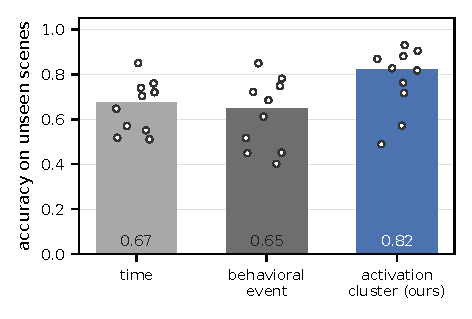
\includegraphics[width=0.9\columnwidth]{figs/fig_readout_bar.pdf}
  \caption{Unseen scene \term{phase} 판독 정확도(instruction 중앙값; 흰 점 = instruction 10개). 회색 = 외부 정보만 쓰는 대조군, 파랑 = 내부 activation.}
  \label{fig:readout}
\end{figure}
\section{결 과}
\textbf{VLA 내부 activation 한 스텝만으로 해당 \term{phase}를 읽을 수 있다.} \rev{Unseen scene에서 측정한 정확도의 instruction 중앙값은 activation 비지도 cluster가 0.82, macro-F1은 0.57이다(Figure~\ref{fig:readout}). 시간 대조군은 정확도 0.61--0.68에 그치고, 외부 관찰로 \term{phase}를 나누는 행동 이벤트 대조군\cite{egsae}은 0.65와 macro-F1 0.37에 그친다.}
\rev{같은 프로토콜에서 activation cluster는 10개 instruction 중 9개에서 행동 이벤트 대조군을 앞서며, 유일한 예외는 모든 방법이 무작위 수준에 머무는 DishwasherRack이다.} 즉 ``에피소드가 얼마나 진행됐는가''도, 밖에서 관찰한 이벤트 구조도 내부 표상만큼은 알려주지 못한다. \rev{특히 비지도 cluster만으로 0.82가 나온다는 점이 중요하다. 구조 자체는 라벨 없이 activation에서 나왔고, 라벨은 각 cluster에 이름을 붙이는 데만 쓰였다.} cluster 중심을 train에서 만들고 평가 스텝은 최근접 배정으로 옮기므로, \rev{다시 clustering하지 않고} 추론 중 스텝 단위로 그대로 돌릴 수 있다.

\textbf{발견된 단위는 사람이 정의한 \term{phase}보다 잘게 나뉜다.} 발견된 상태의 평균 구간 길이는 GT \term{phase}보다 짧고(k=8에서 10개 instruction 전부), 에피소드당 전환 수는 상한($k-1$회)을 모두 넘어 같은 상태를 여러 번 재방문한다.
 \new{다만 이 세분이 의미 있는 하위 구조인지는 본 연구의 범위를 넘는다. \rev{판독 성능은 $k$가 \term{phase} 수를 넘기만 하면 평평하므로($k=8\sim32$에서 0.82--0.88), 앞의 결과는 특정 $k$ 선택에 기대지 않는다.}}

\textbf{각 cluster는 특정 \term{phase}에 국한된다.} 한 \term{phase}에서 나타난 cluster는 다른 \term{phase}에서 잘 나타나지 않는다(Figure 1a). \rev{Cluster를 최빈 \term{phase}로 읽었을 때의 순도 중앙값은 0.875, MI 중앙값은 0.670 bits이며, 시간 대조군 margin의 중앙값은 +0.343 bits로 10개 instruction 전부에서 양수다.} cluster가 최빈 \term{phase} 밖에서 나타나는 비율(\term{off-phase rate})의 중앙값은 0.07이다(instruction별 0.002$\sim$0.45). \new{$k$가 \term{phase} 수보다 크면 실제 \term{phase}보다 많은 cluster가 생기는데, 그런 상황에서도 각 cluster는 특정 \term{phase}에 국한되어 나타나므로 한 \term{phase}를 여러 cluster가 나눠 갖는, 대체로 다대일인 매핑이 된다. \rev{따라서 cluster를 최빈 \term{phase}에 대응시키는 매핑으로 현재 \term{phase}를 읽는 데 지장이 없다. 이것이 세밀한 하위 분할과 \term{phase} 판독이 공존하는 이유다.}}

\textbf{\term{Phase} 정보는 장면 암기로 환원되지 않는다.} \rev{Activation에는 scene 정보도 섞여 있다(instruction별 mi\_scene 0.02$\sim$0.86 bits). 그러나 scene별 평균을 제거한 잔차에서 scene 정보는 중앙값 0.44에서 0.27 bits로 크게 줄어드는 반면, \term{phase} margin은 +0.34에서 +0.31로 10개 instruction 전부에서 양수로 유지된다(Figure 1b).}

\textbf{구조는 모델·데이터를 바꿔도 재현된다.} \rev{별도의 23-에피소드 분석셋에서, 구조가 다른 두 압축 모델(AE와 SAE)이 같은 스텝에서 전환하고}(F1 0.66$\sim$0.75, 무작위 0.51$\sim$0.53, z +8.8$\sim$+13.5), 독립 재수집 데이터에서 새로 학습해도 같은 성질이 나타난다(seed 간 F1 0.55$\sim$0.58, z +4.3$\sim$+5.1). Denoising 슬롯·장면·시드는 에피소드 내 상수라 전환의 원인이 될 수 없다.

% \textbf{세밀 단위는 하류 분석에서도 유용하다.} % 성공/실패 분리도를 단계 조건부로 잴
% 때, 발견 상태(instruction별 k=8)가 GT phase보다 높은 분리도를 주는 instruction이 9개 중
% 4개였다(동급 1, 열세 1; 예: OpenDrawer AUROC 0.93/z4.5 vs GT 0.94/z2.3). 이는 탐색적
% 관찰이나, 세밀 단위가 사람 정의 단계의 단순 잡음이 아님을 시사한다.


\section{한계와 결론}
\textbf{한계.} 평가는 단일 모델(GR00T N1.5)·단일 벤치마크(RoboCasa, 시뮬레이션)에 한정되어 다른 VLA나 실제 로봇으로의 일반화는 확인하지 않았다. GT \term{phase} 라벨은 한 명의 주석자가 부여한 것으로 정확도의 절대값은 주석 기준에 의존하나, 핵심 비교는 모든 방법이 같은 라벨로 채점되므로 영향을 같게 받는다. 마지막으로 본 연구는 내부 표상을 읽을 수 있음(read)을 보인 것이며, 그 표상에 개입해 행동을 바꿀 수 있음(write)은 별개의 검증을 요한다.

\textbf{결론.} VLA의 action head activation에는 사람이 정의한 \term{phase}와 정합적인 구조가 라벨 없이도 드러나며, 이를 이용하면 학습에 쓰지 않은 scene에서도 한 스텝의 activation만으로 \rev{현재 \term{phase}를 정확도 0.82로 읽을 수 있다. 이는 진행 시간(0.67)이나 외부 관찰 기반 행동 이벤트(0.65)로는 닿지 못하는 수준이다.} cluster 중심 최근접 배정만으로 추론 중 스텝 단위 online 판독이 가능하며, \term{phase} 조건부 개입·실패 감지의 조건 신호로 나아가는 출발점이 된다.

% \section*{ACKNOWLEDGMENT}
% TODO: 과제 사사 문구

\renewcommand{\refname}{\centering 참 고 문 헌}
\begin{thebibliography}{99}\scriptsize\setlength{\itemsep}{1pt}\setlength{\parskip}{0pt}
\bibitem{groot} NVIDIA GEAR Team, ``GR00T N1: An Open Foundation Model for
Generalist Humanoid Robots,'' arXiv:2503.14734, 2025.
\bibitem{robocasa} S. Nasiriany et al., ``RoboCasa: Large-Scale Simulation of
Everyday Tasks for Generalist Robots,'' \textit{RSS}, 2024.
\bibitem{saevla} A. Swann et al., ``Sparse Autoencoders Reveal Interpretable and
Steerable Features in VLA Models,'' arXiv:2603.19183, 2026.
\bibitem{observing} H. Buurmeijer et al., ``Observing and Controlling Features in
Vision-Language-Action Models,'' arXiv:2603.05487, 2026.
\bibitem{egsae} X. Jin et al., ``Event-Grounded Sparse Autoencoders for
Vision-Language-Action Policies,'' arXiv:2605.17204, 2026.
\bibitem{awe} L. X. Shi, A. Sharma, T. Z. Zhao, and C. Finn, ``Waypoint-Based
Imitation Learning for Robotic Manipulation,'' \textit{CoRL}, 2023.
\bibitem{siglip} X. Zhai, B. Mustafa, A. Kolesnikov, and L. Beyer, ``Sigmoid Loss
for Language Image Pre-Training,'' \textit{ICCV}, 2023.
\bibitem{mechinterp} B. H\"aon et al., ``Mechanistic Interpretability for Steering
Vision-Language-Action Models,'' \textit{CoRL}, 2025.
\bibitem{safe} Q. Gu et al., ``SAFE: Multitask Failure Detection for
Vision-Language-Action Models,'' \textit{NeurIPS}, 2025.
\bibitem{lotus} W. Wan et al., ``LOTUS: Continual Imitation Learning for Robot
Manipulation Through Unsupervised Skill Discovery,'' \textit{ICRA}, 2024.
\bibitem{options} R. S. Sutton, D. Precup, and S. Singh, ``Between MDPs and
Semi-MDPs: A Framework for Temporal Abstraction in Reinforcement Learning,''
\textit{Artificial Intelligence}, 112:181--211, 1999.
\end{thebibliography}

\end{document}
